\documentclass[11pt]{article}
\usepackage[a4paper,margin=1in]{geometry}
\usepackage{amsmath,amssymb,amsthm}
\usepackage{tikz}
\usepackage{xcolor}
\usepackage[hidelinks]{hyperref}
\hypersetup{pdftitle={Raising the apex},pdfauthor={Vamshi Jandhyala}}
\setlength{\parskip}{0.4em}
\setlength{\parindent}{0pt}

\newtheorem{theorem}{Theorem}
\newtheorem{corollary}{Corollary}
\newtheorem{lemma}{Lemma}
\theoremstyle{remark}
\newtheorem*{remark}{Remark}

\definecolor{inkblue}{RGB}{40,76,105}
\definecolor{softblue}{RGB}{226,235,243}
\definecolor{rust}{RGB}{153,70,45}

\title{Raising the apex raises the Gaussian centroid}
\author{Vamshi Jandhyala}
\date{}

\begin{document}
\maketitle
\vspace{-2em}

\begin{abstract}
Restrict the standard Gaussian measure to a triangle and take its centre of mass. Does the centre of mass
determine the triangle when only one vertex may move? We prove the case in which the moving vertex rises
along the perpendicular to the opposite side through a point of that side: the Gaussian centroid then rises
strictly, in every dimension and over any convex base, wherever the Gaussian is centred. The proof is a
monotone likelihood ratio, supplied by Pr\'ekopa's theorem on log-concave functions. The general case, in which
the vertex moves obliquely and one triangle contains the other, remains open. The steps of the proof after
Pr\'ekopa's theorem are checked in the Lean proof assistant.
\end{abstract}

\section{The question}

Let $\gamma$ be the standard Gaussian density on $\mathbb R^2$. For a triangle $T$ its Gaussian centroid is
\[
e(T)=\frac{\int_T x\,\gamma(x)\,dx}{\int_T\gamma(x)\,dx},
\]
the centre of mass of the Gaussian restricted to $T$. On MathOverflow~\cite{MO}, jens asked whether two
triangles $ABC$ and $ABC'$ with $C'\ne C$ always have different Gaussian centroids, and noted that he needs the
same for $n$-simplices in $\mathbb R^n$. If neither triangle contains the other, a line separates what is
removed from what is added and the centroid shifts across it, as he observes. The hard case is when one
triangle contains the other: the bigger one has extra mass, but the extra mass is far out, where the Gaussian
is small, and it is not obvious that the centroid must move.

Here is the simplest nested case to try before reading on. Keep $A$ and $B$ fixed, put the apex at height $h$
above a point $D$ of the segment $AB$, and raise it. The triangle grows upwards. Does its Gaussian centroid
rise? For the uniform density the centroid height is $h/3$, but the Gaussian may be centred anywhere, even far
to one side, and the new mass lies where the density is small.

\begin{theorem}\label{thm:main}
Let $K$ be a compact convex set with nonempty interior in a hyperplane $H$ of $\mathbb R^n$, $n\ge2$, let
$D\in K$, and let $\nu$ be a unit normal to $H$. For $h>0$ let $T_h$ be the convex hull of $K$ and the apex
$D+h\nu$. Under the standard Gaussian restricted to $T_h$, the mean distance from $H$ is strictly increasing
in $h$.
\end{theorem}

\begin{corollary}\label{cor:tri}
If $C$ and $C'$ are distinct points on the line through a point $D$ of the segment $AB$ perpendicular to $AB$,
and neither equals $D$, then $ABC$ and $ABC'$ have different Gaussian centroids. The same holds for simplices,
with the apex moving along the normal to the opposite facet through a point of that facet.
\end{corollary}

\begin{proof}
On one side of $AB$ apply Theorem~\ref{thm:main} with $K$ the segment $AB$. If $C$ and $C'$ are on opposite
sides, the two centroids are on opposite sides of the line $AB$, since each triangle lies on its own side.
\end{proof}

\begin{figure}[ht]
\centering
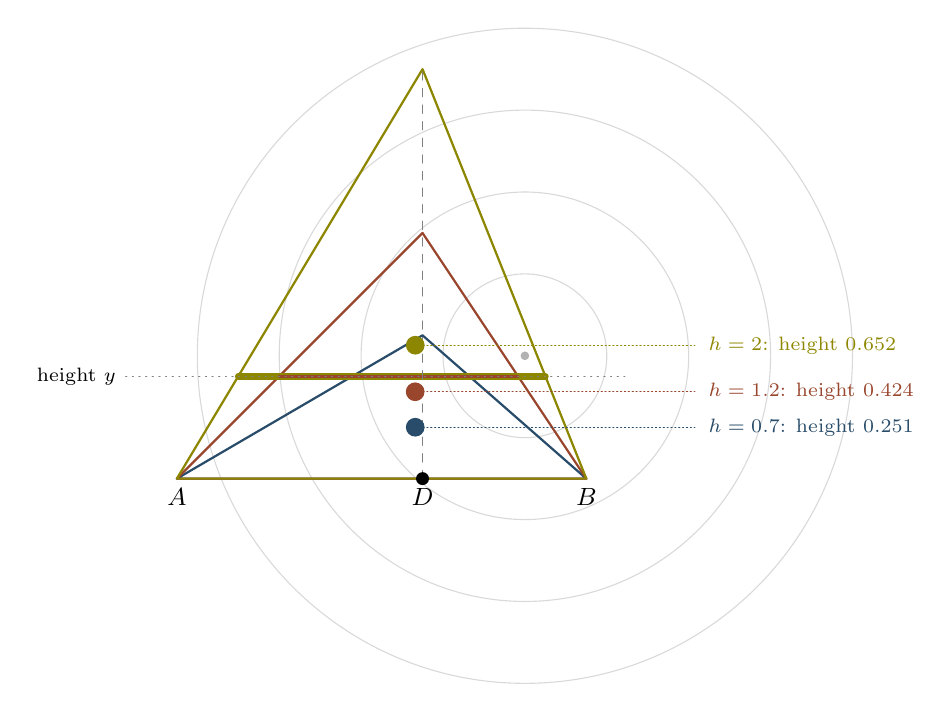
\begin{tikzpicture}[scale=2.6,line cap=round,line join=round]
  \draw[gray!30] (0.5,0.6) circle (0.4);
  \draw[gray!30] (0.5,0.6) circle (0.8);
  \draw[gray!30] (0.5,0.6) circle (1.2);
  \draw[gray!30] (0.5,0.6) circle (1.6);
  \fill[gray!60] (0.5,0.6) circle (0.6pt);
  \draw[inkblue,thick] (-1.2,0) -- (0.8,0) -- (0,0.7) -- cycle;
  \draw[rust,thick] (-1.2,0) -- (0.8,0) -- (0,1.2) -- cycle;
  \draw[olive,thick] (-1.2,0) -- (0.8,0) -- (0,2.0) -- cycle;
  \draw[olive,line width=2.4pt] (-0.9000,0.5) -- (0.6000,0.5);
  \draw[rust,line width=1.2pt] (-0.7000,0.5) -- (0.4667,0.5);
  \draw[gray,dotted] (-1.45,0.5) node[left,font=\scriptsize,black] {height $y$} -- (1.0,0.5);
  \draw[dashed,gray] (0,0) -- (0,2.0);
  \fill (0,0) circle (0.9pt) node[below,font=\small] {$D$};
  \node[below,font=\small] at (-1.2,0) {$A$};
  \node[below,font=\small] at (0.8,0) {$B$};
  \fill[inkblue] (-0.0357,0.2510) circle (1.3pt);
  \node[inkblue,font=\scriptsize,anchor=west] at (1.35,0.2510) {$h=0.7$: height $0.251$};
  \draw[inkblue,densely dotted] (-0.0357,0.2510) -- (1.33,0.2510);
  \fill[rust] (-0.0359,0.4243) circle (1.3pt);
  \node[rust,font=\scriptsize,anchor=west] at (1.35,0.4243) {$h=1.2$: height $0.424$};
  \draw[rust,densely dotted] (-0.0359,0.4243) -- (1.33,0.4243);
  \fill[olive] (-0.0355,0.6517) circle (1.3pt);
  \node[olive,font=\scriptsize,anchor=west] at (1.35,0.6517) {$h=2$: height $0.652$};
  \draw[olive,densely dotted] (-0.0355,0.6517) -- (1.33,0.6517);
\end{tikzpicture}

\caption{Three apexes above the foot $D$ and the Gaussian contours, centred off the axis of symmetry. The slice
at height $y$ of each triangle is the base shrunk towards $D$ by the factor $1-y/h$. The Gaussian centroids
(dots, computed by quadrature) rise with $h$.}
\label{fig:slices}
\end{figure}

The theorem needs no symmetry of the base or of the Gaussian: $D$ may be anywhere in $K$, and the Gaussian may
be centred anywhere. Two of its hypotheses cannot be dropped. If the foot is outside the base, the mean height
can fall: for $A=(10,0)$, $B=(11,0)$ and apex $(0,h)$, the mean height is about $5.050$ at $h=10$ and $4.048$
at $h=20$. And the proof uses log-concavity in an essential way, as the remark after Lemma~\ref{lem:ratio}
explains.

\section{Proof}

Take coordinates $(x,y)$ with $x\in H$ and $y$ the signed distance from $H$. The standard Gaussian density
factors as $\rho(x)\,w(y)$, with $\rho$ a Gaussian density on $H$ and $w$ a one-dimensional one, because $H$
and $\nu$ are orthogonal. The section of $T_h$ at height $y\in(0,h)$ is the base shrunk towards $D$:
\[
D+s(K-D),\qquad s=1-\frac yh .
\]
So the height of a Gaussian point of $T_h$ has density proportional to
\[
q_h(y)=w(y)\,F\Bigl(1-\frac yh\Bigr)\quad(0<y<h),\qquad F(s)=\int_{D+s(K-D)}\rho(x)\,dx .
\]
Read $F(s)$ as the Gaussian mass of the base scaled by $s$ about $D$. Everything depends on two properties of
$F$.

\emph{$F$ is strictly increasing.} As $D\in K$ and $K$ is convex, the scaled copies are nested, and their
volumes $s^{n-1}\operatorname{vol}(K)$ grow strictly; $\rho$ is positive.

\emph{$\log F$ is concave.}

\begin{lemma}\label{lem:cone}
For $s_1,s_2>0$, $0\le\lambda\le1$ and $z_1,z_2\in K$,
\[
(1-\lambda)\bigl(D+s_1(z_1-D)\bigr)+\lambda\bigl(D+s_2(z_2-D)\bigr)=D+s(z-D)
\]
for $s=(1-\lambda)s_1+\lambda s_2$ and some $z\in K$.
\end{lemma}

\begin{proof}
Take $z=a z_1+b z_2$ with $a=(1-\lambda)s_1/s$ and $b=\lambda s_2/s$, which are
nonnegative and sum to $1$; then $s(z-D)=(1-\lambda)s_1(z_1-D)+\lambda s_2(z_2-D)$.
\end{proof}

So the set $\mathcal C=\{(x,s):s>0,\ x\in D+s(K-D)\}$ is convex, the function $(x,s)\mapsto\rho(x)\mathbf
1_{\mathcal C}(x,s)$ is log-concave, and by Pr\'ekopa's theorem~\cite[Theorem~6]{Pre73} its integral over $x$,
which is $F(s)$, is log-concave.

\begin{lemma}\label{lem:ratio}
Let $\varphi$ be concave and strictly increasing on $(0,\infty)$, and $0<h_1<h_2$. Then
\[
y\;\longmapsto\;\varphi\Bigl(1-\frac y{h_2}\Bigr)-\varphi\Bigl(1-\frac y{h_1}\Bigr)
\]
is strictly increasing on $(0,h_1)$.
\end{lemma}

\begin{proof}
Let $y<y'$. As $y$ moves to $y'$, the argument $1-y/h_1$ runs back over an interval of length $(y'-y)/h_1$,
and $1-y/h_2$ over a shorter interval, of length $(y'-y)/h_2$, that starts no lower. A concave function gains
no more over an interval of given length the further right it lies: writing $u_2$ and $u_1+L$ as complementary
convex combinations of $u_1$ and $u_2+L$ and adding the two concavity inequalities gives
$\varphi(u_2+L)-\varphi(u_2)\le\varphi(u_1+L)-\varphi(u_1)$ for $u_1\le u_2$. A strictly increasing function
gains strictly more over a longer interval with the same left end. Together, $\varphi$ loses strictly more along
the first argument than along the second, which is the claim.
\end{proof}

Apply it with $\varphi=\log F$: the likelihood ratio $r(y)=q_{h_2}(y)/q_{h_1}(y)=F(1-y/h_2)/F(1-y/h_1)$ is
strictly increasing on $(0,h_1)$. The factor $w(y)$ has cancelled, which is why the Gaussian may be centred
anywhere.

\begin{remark}
Without log-concavity the ratio need not increase. For $F(s)=se^{50s^2}$, which is increasing, the derivative
of $\log r$ at $h_1=1$, $h_2=2$, $y=\frac45$ is $-\frac{35}6$.
\end{remark}

\begin{proof}[Proof of Theorem~\ref{thm:main}]
Let $0<h_1<h_2$ and let $\mu$ be the height law for $h_1$, with density proportional to $q_{h_1}$ on $(0,h_1)$.
The law for $h_2$, conditioned on $(0,h_1)$, has density proportional to $r\,q_{h_1}$, so its mean is
$\int yr\,d\mu\big/\!\int r\,d\mu$. Chebyshev's integral inequality for the two increasing functions $y$ and $r$
says
\[
\int y\,d\mu\int r\,d\mu<\int yr\,d\mu ,
\]
strictly because $(y-y')(r(y)-r(y'))>0$ whenever $y\ne y'$, and $\mu\otimes\mu$ gives the diagonal no mass. (The
proof is one line: the double integral of $(y-y')(r(y)-r(y'))$ is positive and equals
$2(\int yr-\int y\int r)$ for a probability measure.) So the conditional mean exceeds the mean for $h_1$. The
rest of the $h_2$ law lies in $[h_1,h_2)$, above both, so the mean for $h_2$ is larger still.
\end{proof}

\begin{remark}
The proof gives more than the means: the height laws increase in the likelihood-ratio order. It also works for
any positive log-concave density in place of $\rho$ and any positive weight $w(y)$, which cancels. It does not
reach the general nested case. When the apex moves obliquely, the sections are no longer scaled copies of the
base about a fixed point, so the height laws are not all built from one function $F$, and the likelihood-ratio
comparison has nothing to hold on to. Whether the Gaussian centroid determines the moving vertex in general
remains open.
\end{remark}

\paragraph{Verification.} Lemma~\ref{lem:cone}, the increment inequality and Lemma~\ref{lem:ratio},
Chebyshev's integral inequality with its strict form for any finite measure on $\mathbb R$, and the final
comparison of means are checked in Lean~4 with Mathlib~\cite{mathlib}, using only the standard axioms. Quoted
rather than formalised: Pr\'ekopa's theorem, the factorisation of the Gaussian and the resulting height
densities, and the strict increase of $F$. A Python program audits the section identities, the likelihood
ratios, the means and the two counterexamples by quadrature, and deliberately wrong variants fail it; an
independent program, sharing no code with it, computes Gaussian centroids of triangles and of a tetrahedron by
Monte Carlo and checks that they rise with the apex. Everything is at
\url{https://github.com/jvvk/mathematics/tree/main/raising-the-apex}.

\paragraph{Acknowledgements.} jens asked the question. Anthropic's Claude (Opus~5.5) was used to find the
argument, write the Lean formalisation and the programs, and draft this text. The author takes responsibility
for the content.

\begin{thebibliography}{9}
\bibitem{MO} jens, Gaussian expectation on a triangle is one-to-one with any single vertex?, MathOverflow
question 499635 (26 August 2025), \url{https://mathoverflow.net/q/499635}, accessed 10 October 2026.
\bibitem{Pre73} A.~Pr\'ekopa, On logarithmic concave measures and functions, \emph{Acta Sci. Math. (Szeged)}
\textbf{34} (1973) 335--343.
\bibitem{mathlib} The mathlib Community, The Lean mathematical library, in \emph{Proceedings of the 9th ACM
SIGPLAN International Conference on Certified Programs and Proofs (CPP 2020)}, 367--381,
\href{https://doi.org/10.1145/3372885.3373824}{doi:10.1145/3372885.3373824}.
\end{thebibliography}

\bigskip
\noindent Vamshi Jandhyala, London, UK.

\end{document}
